\documentclass[journal,12pt,twocolumn]{IEEEtran}

\usepackage{setspace}
\usepackage{gensymb}
\singlespacing
\usepackage[cmex10]{amsmath}

\usepackage{amsthm}

\usepackage{mathrsfs}
\usepackage{txfonts}
\usepackage{stfloats}
\usepackage{bm}
\usepackage{cite}
\usepackage{cases}
\usepackage{subfig}

\usepackage{longtable}
\usepackage{multirow}

\usepackage{enumitem}
\usepackage{mathtools}
\usepackage{steinmetz}
\usepackage{tikz}
\usepackage{circuitikz}
\usepackage{verbatim}
\usepackage{tfrupee}
\usepackage[breaklinks=true]{hyperref}
\usepackage{graphicx}
\usepackage{tkz-euclide}

\usetikzlibrary{calc,math}
\usepackage{listings}
    \usepackage{color}                                            %%
    \usepackage{array}                                            %%
    \usepackage{longtable}                                        %%
    \usepackage{calc}                                             %%
    \usepackage{multirow}                                         %%
    \usepackage{hhline}                                           %%
    \usepackage{ifthen}                                           %%
    \usepackage{lscape}     
\usepackage{multicol}
\usepackage{chngcntr}

\DeclareMathOperator*{\Res}{Res}

\renewcommand\thesection{\arabic{section}}
\renewcommand\thesubsection{\thesection.\arabic{subsection}}
\renewcommand\thesubsubsection{\thesubsection.\arabic{subsubsection}}

\renewcommand\thesectiondis{\arabic{section}}
\renewcommand\thesubsectiondis{\thesectiondis.\arabic{subsection}}
\renewcommand\thesubsubsectiondis{\thesubsectiondis.\arabic{subsubsection}}
\newtheorem{theorem}{Theorem}[section]
\newtheorem{corollary}{Corollary}[theorem]
\newtheorem{lemma}[theorem]{Lemma}
\newtheorem{definition}{Definition}[section]


\hyphenation{op-tical net-works semi-conduc-tor}
\def\inputGnumericTable{}                                 %%

\lstset{
%language=C,
frame=single, 
breaklines=true,
columns=fullflexible
}
\begin{document}

\newcommand{\BEQA}{\begin{eqnarray}}
\newcommand{\EEQA}{\end{eqnarray}}
\newcommand{\define}{\stackrel{\triangle}{=}}
\bibliographystyle{IEEEtran}
\raggedbottom
\setlength{\parindent}{0pt}
\providecommand{\mbf}{\mathbf}
\providecommand{\pr}[1]{\ensuremath{\Pr\left(#1\right)}}
\providecommand{\qfunc}[1]{\ensuremath{Q\left(#1\right)}}
\providecommand{\sbrak}[1]{\ensuremath{{}\left[#1\right]}}
\providecommand{\lsbrak}[1]{\ensuremath{{}\left[#1\right.}}
\providecommand{\rsbrak}[1]{\ensuremath{{}\left.#1\right]}}
\providecommand{\brak}[1]{\ensuremath{\left(#1\right)}}
\providecommand{\lbrak}[1]{\ensuremath{\left(#1\right.}}
\providecommand{\rbrak}[1]{\ensuremath{\left.#1\right)}}
\providecommand{\cbrak}[1]{\ensuremath{\left\{#1\right\}}}
\providecommand{\lcbrak}[1]{\ensuremath{\left\{#1\right.}}
\providecommand{\rcbrak}[1]{\ensuremath{\left.#1\right\}}}
\theoremstyle{remark}
\newtheorem{rem}{Remark}
\newcommand{\sgn}{\mathop{\mathrm{sgn}}}
\providecommand{\abs}[1]{\vert#1\vert}
\providecommand{\res}[1]{\Res\displaylimits_{#1}} 
\providecommand{\norm}[1]{\lVert#1\rVert}
%\providecommand{\norm}[1]{\lVert#1\rVert}
\providecommand{\mtx}[1]{\mathbf{#1}}
\providecommand{\mean}[1]{E[ #1 ]}
\providecommand{\fourier}{\overset{\mathcal{F}}{ \rightleftharpoons}}
%\providecommand{\hilbert}{\overset{\mathcal{H}}{ \rightleftharpoons}}
\providecommand{\system}{\overset{\mathcal{H}}{ \longleftrightarrow}}
	%\newcommand{\solution}[2]{\textbf{Solution:}{#1}}
\newcommand{\solution}{\noindent \textbf{Solution: }}
\newcommand{\cosec}{\,\text{cosec}\,}
\providecommand{\dec}[2]{\ensuremath{\overset{#1}{\underset{#2}{\gtrless}}}}
\newcommand{\myvec}[1]{\ensuremath{\begin{pmatrix}#1\end{pmatrix}}}
\newcommand{\mydet}[1]{\ensuremath{\begin{vmatrix}#1\end{vmatrix}}}
\numberwithin{equation}{subsection}
\makeatletter
\@addtoreset{figure}{problem}
\makeatother
\let\StandardTheFigure\thefigure
\let\vec\mathbf
\renewcommand{\thefigure}{\theproblem}
\def\putbox#1#2#3{\makebox[0in][l]{\makebox[#1][l]{}\raisebox{\baselineskip}[0in][0in]{\raisebox{#2}[0in][0in]{#3}}}}
     \def\rightbox#1{\makebox[0in][r]{#1}}
     \def\centbox#1{\makebox[0in]{#1}}
     \def\topbox#1{\raisebox{-\baselineskip}[0in][0in]{#1}}
     \def\midbox#1{\raisebox{-0.5\baselineskip}[0in][0in]{#1}}
\vspace{3cm}
\title{ EE3900 : Gate Assignment-4}
\author{Nelakuditi Rahul Naga - AI20BTECH11029}
\maketitle
\newpage
\bigskip
\renewcommand{\thefigure}{\theenumi}
\renewcommand{\thetable}{\theenumi}
Download all latex tikz codes from 
\begin{lstlisting}
https://github.com/Rahul27n/EE3900/blob/main/Gate_Assignment_4/Gate_Assignment_4.tex
\end{lstlisting}
\vspace{0.5cm}
\section{QUESTION: GATE EC 1998 Q1.4}
The trigonometric Fourier series of a periodic time function can have only:
\begin{enumerate}[label=(\Alph*)]
\item cosine terms 
\item sine terms
\item d.c. ,cosine and sine terms
\item d.c. and cosine terms 
\end{enumerate}
\section{SOLUTION}
The trigonometric Fourier series of a periodic function $x(t)$ with period $T$ is given by:
\begin{align}
x(t) &= a_{0} + \sum_{k=1}^{\infty}a_{k}\cos{\frac{2\pi kt}{T}} +\sum_{k=1}^{\infty}b_{k}\sin{\frac{2\pi kt}{T}}
\end{align}
where $a_{0}$ is the d.c component of the signal and $a_{k}$ and $b_{k}$ are Fourier coefficients. The Fourier series of some example functions are given by:
\begin{enumerate}
\item We have a even periodic function having period $2\pi$ defined in $[-\pi,\pi]$ as follows :
\begin{align}
x(t)=  
\begin{cases}
\frac{\pi}{2}+t, & \text{if } -\pi \leq t \leq 0\\
\frac{\pi}{2}-t, & \text{if } 0 < t \leq \pi \nonumber
\end{cases}
\end{align}
The Fourier series of $x(t)$ is determined as follows:
\begin{align}
a_{0} &=\frac{1}{2\pi}\Bigg({\int_{-\pi}^{0}x(t)\, dt}+{\int_{0}^{\pi}x(t)\, dt}\Bigg)=0 \nonumber \\
a_{k} &= \frac{1}{\pi}\Bigg({\int_{-\pi}^{0}x(t)\cos{kt}\, dt}+{\int_{0}^{\pi}x(t)\cos{kt}\, dt}\Bigg) \nonumber \\
&= \frac{2(1-(-1)^{k})}{\pi k^{2}}\nonumber \\
b_{k} &= \frac{1}{\pi}{\int_{-\pi}^{\pi}x(t)\sin{kt}\, dt} = 0\nonumber
\end{align}
\begin{align}
x(t) &= \frac{4}{\pi}\sum_{k=1}^{\infty}\frac{\cos{(2k-1)t}}{(2k-1)^{2}}
\end{align}
\begin{figure}[!ht]
    \centering
    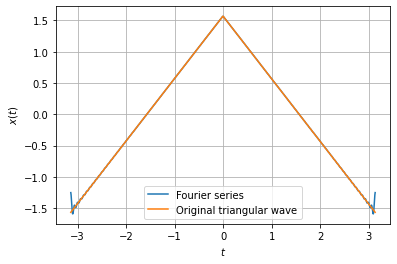
\includegraphics[width=\columnwidth] {Gate_Assignment_4_Fig_1.png}
    \caption{$x(t)$ vs $t$}
    \label{Fourier series of x(t)}
\end{figure}
\item We have a odd periodic function having period $2\pi$ defined in $[0,2\pi]$ as follows :
\begin{align}
x(t)=  
\begin{cases}
1, & \text{if } 0 < t < \pi\\
0, & \text{if } t = 0,\pi,2\pi\\
-1, & \text{if } \pi < t < 2\pi \nonumber
\end{cases}
\end{align}
The Fourier series of $x(t)$ is determined as follows:
\begin{align}
a_{0} &=\frac{1}{2\pi}{\int_{-\pi}^{\pi}x(t)\, dt}=0 \nonumber \\
a_{k} &= \frac{1}{\pi}{\int_{-\pi}^{\pi}x(t)\cos{kt}\, dt} = 0\nonumber \\
b_{k} &= \frac{1}{\pi}\Bigg({\int_{-\pi}^{0}x(t)\sin{kt}\, dt}+{\int_{0}^{\pi}x(t)\sin{kt}\, dt}\Bigg) \nonumber \\
&= \frac{2(1-(-1)^{k})}{\pi k}\nonumber \\
x(t) &= \frac{4}{\pi}\sum_{k=1}^{\infty}\frac{\sin{(2k-1)t}}{2k-1}
\end{align}
\begin{figure}[!ht]
    \centering
    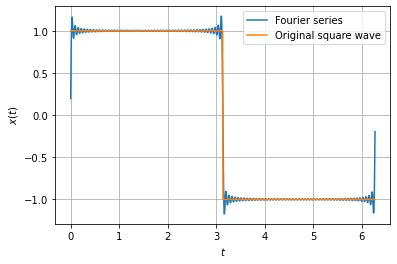
\includegraphics[width=\columnwidth] {Gate_Assignment_4_Fig_2.png}
    \caption{$x(t)$ vs $t$}
    \label{Fourier series of x(t)}
\end{figure}
\item We have a neither even nor odd periodic function having period $2\pi$ defined in $(-\pi,\pi)$ as follows :
\begin{align}
x(t)=  
\begin{cases}
-\pi, & \text{if } -\pi < t < 0\\
-\frac{\pi}{2}, & \text{if } t=0\\
t, & \text{if } 0 < t < \pi \nonumber
\end{cases}
\end{align}
The Fourier series of $x(t)$ is determined as follows:
\begin{align}
a_{0} &=\frac{1}{2\pi}\Bigg({\int_{-\pi}^{0}x(t)\, dt}+{\int_{0}^{\pi}x(t)\, dt}\Bigg)= -\frac{\pi}{4} \nonumber \\
a_{k} &= \frac{1}{\pi}\Bigg({\int_{-\pi}^{0}x(t)\cos{kt}\, dt}+{\int_{0}^{\pi}x(t)\cos{kt}\, dt}\Bigg) \nonumber \\
&= \frac{(-1)^{k}-1}{\pi k^{2}}\nonumber
\end{align}
\begin{align}
b_{k} &= \frac{1}{\pi}\Bigg({\int_{-\pi}^{0}x(t)\sin{kt}\, dt}+{\int_{0}^{\pi}x(t)\sin{kt}\, dt}\Bigg) \nonumber \\
&= \frac{2(-1)^{k}+1}{k}\nonumber \\
x(t) &= -\frac{\pi}{4}-\frac{2}{\pi}\sum_{k=1}^{\infty}\frac{\cos{(2k-1)t}}{(2k-1)^{2}}+\sum_{k=1}^{\infty}b_{k}\sin{kt}
\end{align}
\begin{figure}[!ht]
    \centering
    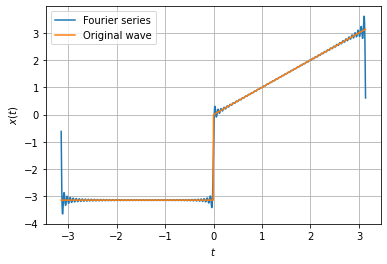
\includegraphics[width=\columnwidth] {Gate_Assignment_4_Fig_3.png}
    \caption{$x(t)$ vs $t$}
    \label{Fourier series of x(t)}
\end{figure}
\item We have a even periodic function having period $2\pi$ defined in $(0,2\pi)$ as follows :
\begin{align}
x(t)=  
\begin{cases}
t, & \text{if } 0 < t \leq \pi\\
2\pi-t, & \text{if } \pi \leq  t <  2\pi \nonumber
\end{cases}
\end{align}
The Fourier series of $x(t)$ is determined as follows:
\begin{align}
a_{0} &=\frac{1}{2\pi}\Bigg({\int_{-\pi}^{0}x(t)\, dt}+{\int_{0}^{\pi}x(t)\, dt}\Bigg)= \frac{\pi}{2} \nonumber \\
a_{k} &= \frac{1}{\pi}\Bigg({\int_{-\pi}^{0}x(t)\cos{kt}\, dt}+{\int_{0}^{\pi}x(t)\cos{kt}\, dt}\Bigg) \nonumber \\
&= \frac{2((-1)^{k}-1)}{\pi k^{2}}\nonumber \\
b_{k} &= \frac{1}{\pi}{\int_{-\pi}^{\pi}x(t)\sin{kt}\, dt} = 0\nonumber \\
x(t) &= \frac{\pi}{2}-\frac{4}{\pi}\sum_{k=1}^{\infty}\frac{\cos{(2k-1)t}}{(2k-1)^{2}}
\end{align}
\end{enumerate}
\begin{figure}[!ht]
    \centering
    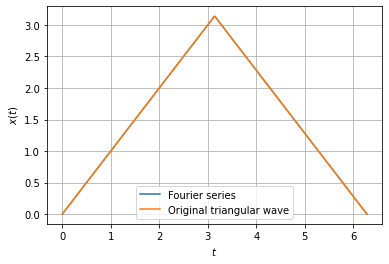
\includegraphics[width=\columnwidth] {Gate_Assignment_4_Fig_4.png}
    \caption{$x(t)$ vs $t$}
    \label{Fourier series of x(t)}
\end{figure}
Hence the correct answer is option (C).
\end{document}
